\chapter{Proposed Translator}
\label{ch:proposed-system}

Para solucionar el problema expuesto en el punto 4, con toda esa información
proponemos una sintaxis basada en shexc que representa el subconjunto que podemos representar con PO.
Dicha sintaxis a demás al ser un subconjunto está validada semantica y sintácticamente de forma que
tiene más restricciones que shex normal, de forma que se aseguran las integridades del lenguage y
se propone un sistema de errores "actualizado". Para esta sintaxis ofrecemos tb un compilador
diseñado como una API que compila los esquemas que se realzian en esta sintaxis y los traduce al
lenguaje de programación objetivo que se desee.

\section{Structure}

\section{Generated Obejcts}

\begin{figure}
    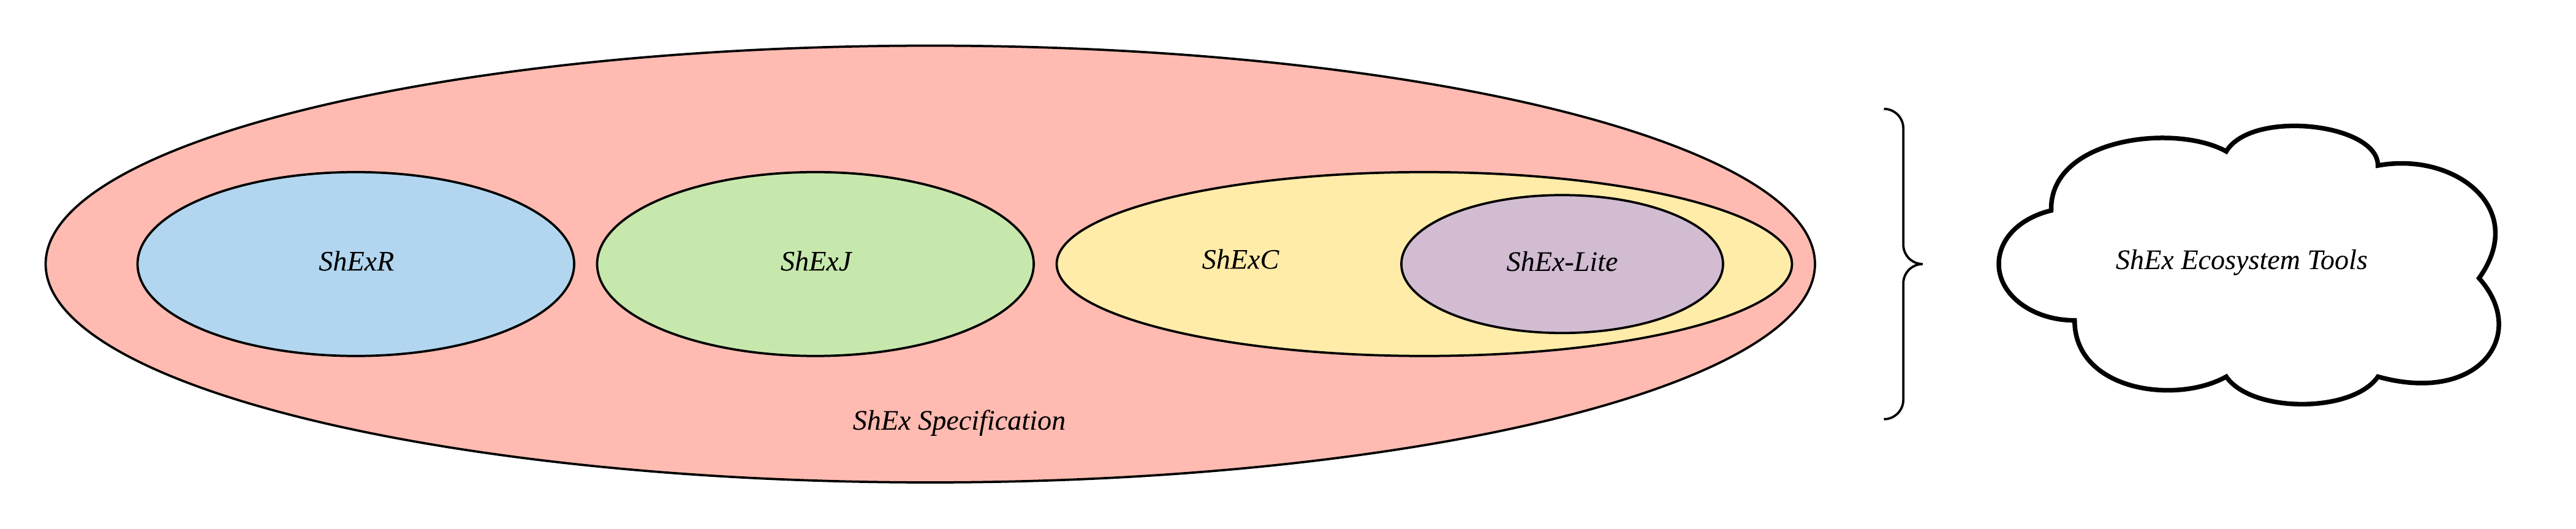
\includegraphics[width=\textwidth]{images/shex-lite-syntaxes-mental-model.png}
    \centering
    \caption[Mental model of ShEx-Lite in the existing ShEx syntaxes context.]{Mental model of
    ShEx-Lite in the existing ShEx syntaxes context. From this model we can see that Shex-Lite
    is in fact an strictly subset of ShExC, which follows the ShEx Specification. And therefore
    ShEx-Lite will also follow that expecification, which automatically enables ShEx-Lite schemas
    to be used in any other existing ShEx tool.}
    \label{fig:syntax-mental-model}
\end{figure}

\begin{figure}
  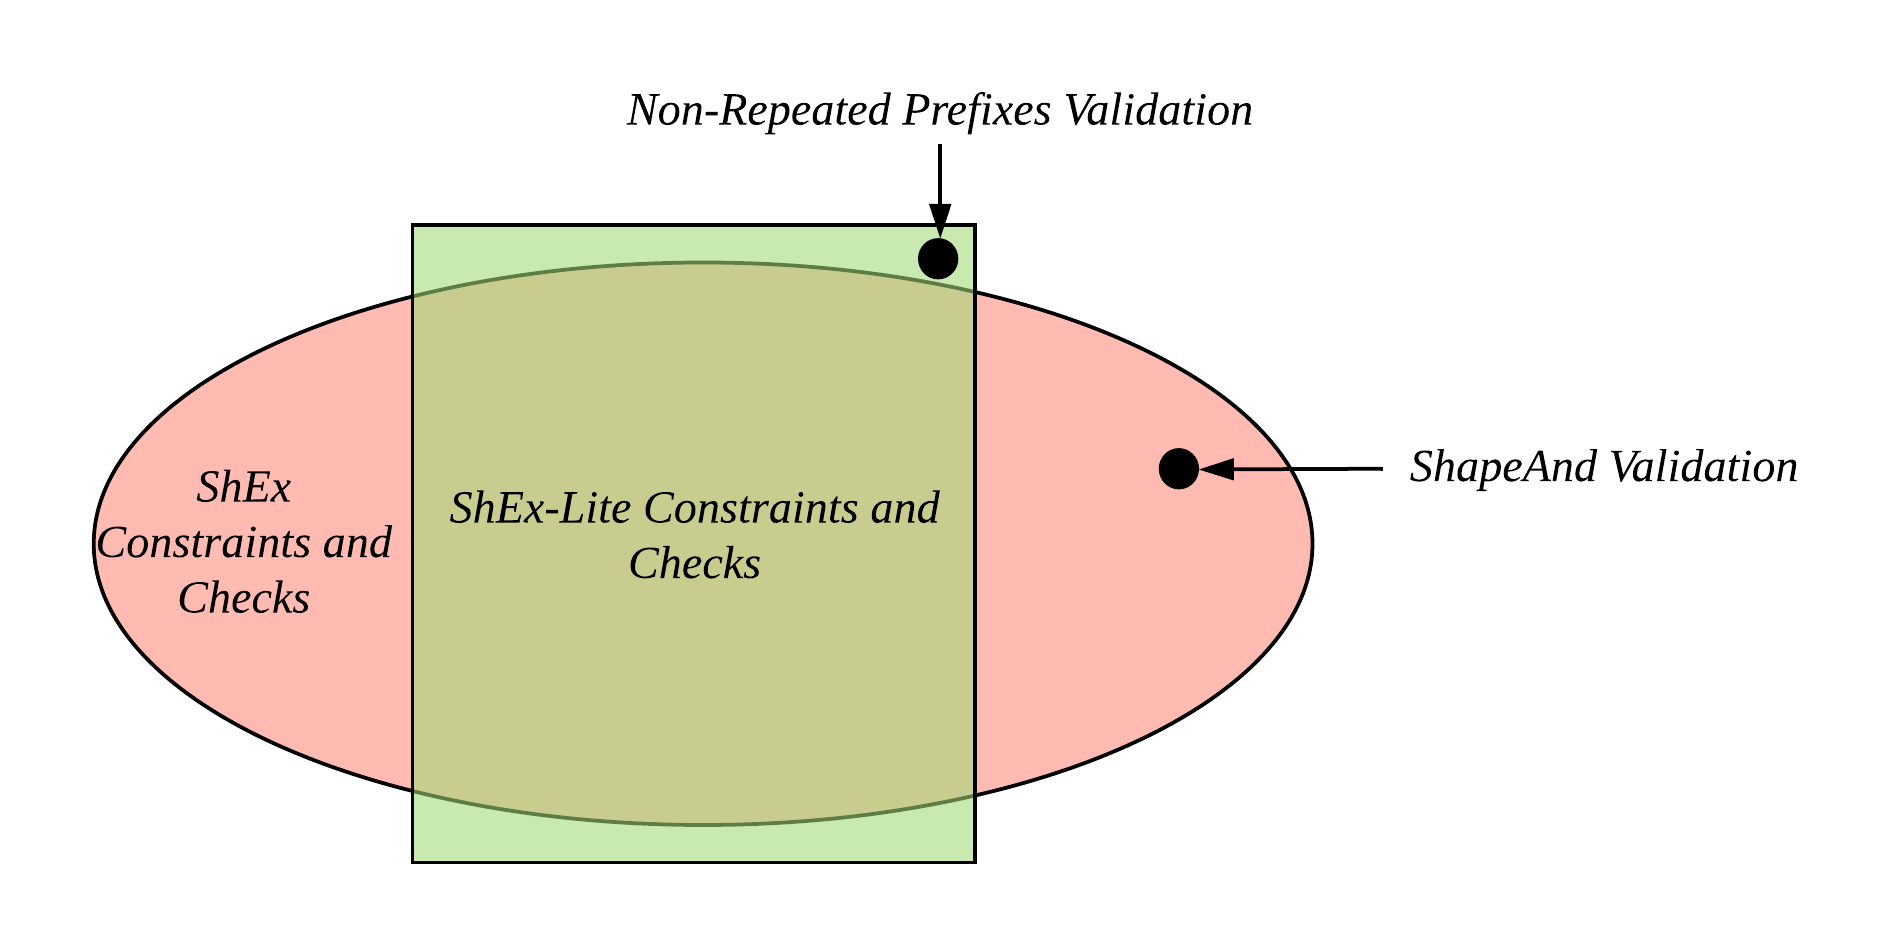
\includegraphics[width=\textwidth]{images/shex-lite-constraints-context.png}
  \centering
  \caption[Constraints and checks context diagram for ShEx-Lite and ShEx.]{Constraints
  and checks context diagram for ShEx-Lite and ShEx.}
  \label{fig:constraints-context}
\end{figure}

\begin{center}
	\noindent\begin{minipage}[t]{.4\textwidth}
		\begin{lstlisting}[frame=topline,numbers=left,title=\scriptsize\texttt{Person.shexl}, basicstyle=\ttfamily\scriptsize]{a}
# Prefixes...
:Person {
	:name xsd:string ;
	:knows @:Person *
}
		\end{lstlisting}
	\end{minipage}\hfill
	\begin{minipage}[t]{.5\textwidth}
		\begin{lstlisting}[language=Java, frame=t,numbers=left,title=\scriptsize\texttt{Person.java}, basicstyle=\ttfamily\scriptsize]{b}
// Imports...
public class Person {
	private String name;
	private List<Person> knows;
	// Constructor...
	// Getters and Setters...
}
		\end{lstlisting}
	\end{minipage}
	\captionof{figure}{Schema modeling a \texttt{Person} in \texttt{shexl} syntax to the left. And the \texttt{ShEx-Lite} generated code in \texttt{Java} to the right.}
	\label{fig:example-1}
\end{center}